\section{Funktionsweise von Vektoruhren}
\subsection{Prinzipielle Funktionsweise}

Wie bereits beschrieben wurde, bilden Vektoruhren eine Erweiterung der Lamportuhr. Dabei wird pro Node im System ein Integer als Zähler für den Node in der Vektoruhr gespeichert. Im Allgemeinen werden durch eine Vektoruhr Zeitstempel mit Events im System assoziiert \cite{Baldoni:2002:FDC:1435723.1437765}[S. 3].

Jeder Node im System besitzt seine eigene Vektoruhr in der Form eines Vektors $VC_i[1...n]$, wobei alle Elemente der Uhr mit $0$ initialisiert werden. Die Uhr eines Nodes wird wie folgt verwaltet und aktualisiert:

\begin{itemize}
	\item[R1]Jedes mal, wenn ein Node $P_i$ ein Event auslöst, muss dieser seine Vektoruhr für den Eintrag $VC_i$ um Eins hochzählen, es gilt  $VC_i[i] := VC_i[i] + 1$. Dadurch verdeutlicht der Node, dass er etwas getan hat und signalisiert dies den anderen Nodes durch aktualisieren seiner Vektoruhr 
	\item[R2]Sendet ein Node $P_i$ eine Nachricht $m$, so hängt er seine aktuelle Vektoruhr $VC_i$ an die zu sendende Nachricht an. Auf diese Weise gelangt die Uhr zu dem Empfänger der Nachricht.
	\item[R3]Empfängt ein Node $P_i$ eine Nachricht, so muss er seine Vektoruhr aktualisieren. Dabei geht er wie folgt vor: $VC_i = \max(VC_i, m.VC)$. Dies bedeutet, dass der Node für jedes Element seiner Vektoruhr überprüft ob der Wert in der Uhr der Nachricht größer als der eigene ist. Sollte dies der Fall sein, wird der eigene Wert an dieser Stelle mit dem Wert aus der anderen Uhr überschrieben.\label{R3}
\end{itemize} \cite{Baldoni:2002:FDC:1435723.1437765}[S. 4]

Die Werte innerhalb einer Vektoruhr $VC_i$ haben eine besondere Bedeutung für den Node $P_i$. $VC_i[i]$ gibt die Anzahl an Events an, welche $P_i$ zu dem Zeitpunkt des Betrachtens verarbeitet hat. Die anderen Werte der Uhr ($VC_i[j]$ mit $j \neq i$) zeigen an, dass alle Events welche durch den Node $P_j$ verarbeitet wurden, sich kausal betrachtet in der Vergangenheit von $P_i$ befinden. Sie geben sozusagen an, was Node $P_i$ über die Zeiten der anderen Nodes weiß, diese Information kann sich zu dem Zeitpunkt jedoch bereits von den tatsächlichen Zeiten unterscheiden. Da jeder Node lediglich seinen Zähler in der Vektoruhr erhöhen darf, hat dieser Node zu jedem Zeitpunkt den aktuellsten Stand seiner lokalen Zeit. \cite{SINGHAL199247}[S. 48]

\subsubsection{Vergleich von Vektoruhren untereinander}
Eine Besonderheit der Vektoruhren besteht im Vergleich von Uhren untereinander. Dies wird notwendig, sobald ein Node eine Nachricht erhält und diese verarbeiten muss. Wie in Bedingung R3 unter \ref{R3} - \nameref{R3} zu sehen, muss der Node seine Uhr entsprechen der mitgeschickten Vektoruhr der Nachricht aktualisieren. Der Vergleich zwischen der eigenen und der empfangenen Uhr muss dann auf Anwendungsebene geschehen, denn dort wird entschieden was mit der angekommenen Nachricht geschieht.

Für zwei zu vergleichende Uhren $VC_1$ und $VC_2$ gibt es folgenden Beziehungen:

\begin{eqnarray}
&VC_1 \leq VC_2& \text{ wenn } \forall i : VC_1[i] \leq VC_2[i] \\
	&VC_1 < VC_2& \text{ wenn } VC_1 \leq VC_2 \text{ \& } VC_1 \neq VC_2 \\
	&VC_1 \mid \mid VC_2& \text{ wenn } !(VC_1 < VC_2) \text{ \& } !(VC_2 < VC_1)
\end{eqnarray}
\cite{Mattern88virtualtime}[S. 127, Definition 4]

Fall (1) bedeutet, dass eine Uhr $VC_1$ kleiner oder gleich $VC_2$ ist, wenn jedes Element von $VC_1$ kleiner oder gleich dem entsprechenden Element in $VC_2$ ist. Der zweite Fall (2) liegt vor, wenn Fall (1) zutrifft und zusätzlich kein Element in $VC_1$ gleich dem entsprechenden Element in $VC_2$ ist. 
Der letzte Fall (3) ist ein Besonderer Fall. Dieser trifft ein wenn nicht entschieden werden kann, welche Uhr neuer oder älter beziehungsweise nach der obigen Definition größer oder kleiner ist als die andere. Die entsprechenden Nachrichten wurden sozusagen gleichzeitig abgeschickt. Dieser im Englischen als Concurrent bezeichnete Fall stellt ein großes Problem für Systeme dar, die Vektoruhren für die zeitliche Synchronisation der Kommunikation nutzen. Auf diesen Sonderfall wird im nächsten Kapitel genauer eingegangen.
\subsubsection{Beispiel einer Kommunikation}
Um die Funktionsweise von Vektoruhren genauer zu beschreiben, wird nun anhand eines einfachen Beispieles die Kommunikation in einem System mit drei Nodes sowie die Verarbeitung der Vektoruhren eines jeden Nodes gezeigt.

TODO: Beispiel schrittweise zeigen und Uhren beschreiben

\subsection{Umsetzung in C\#}
Für die Umsetzung dieses Themas wurde C\# als Programmiersprache ausgewählt. Damit die zeitliche Synchronisation mittels Vektoruhren möglichst realitätsnah simuliert werden kann, wurden drei virtuelle Maschinen mit dem Betriebssystem Windows 8.1 aufgesetzt. Diese befinden sich im Hochschulnetzwerk und können per Remote Desktop bedient werden.

Die Implementierung wurde in zwei unabhängige Programmteile aufgeteilt. Diese sind ein Commander sowie Nodes. 

TODO: Abbildung des Gesamtsystemes (Commander + 3 Nodes)

Der Commander stellt sozusagen eine übergeordnete Kommandozentrale dar, welche die Kommunikation der Nodes untereinander durch gewisse Steuerbefehle koordiniert. Er besitzt eine grafische Oberfläche, welche mittels WPF erstellt wurde.

\begin{figure}[ht]
	\centering
	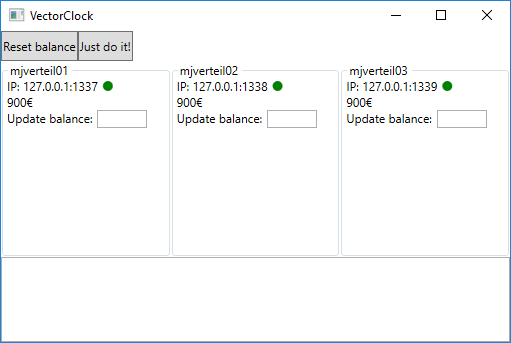
\includegraphics[width=10cm]{commanderWindow.png}
	\caption[Commander Window]{Abbildung des Commanderfensters, welcher dazu dient, die Kommunikation zwischen den Nodes durch Steuerbefehle zu koordinieren}}
	\label{figure:commanderWindow}
\end{figure}
\FloatBarrier

Ein Node stellt einen Knoten in dem simulierten System dar. In diesem werden Events ausgeführt und Vektoruhren verarbeitet. Jeder Node besitzt seine eigene, lokale Vektoruhr. Bei einem Node handelt es sich um ein Kommandozeilenprogramm, welches auf einer VM läuft und ständig auf Nachrichten wartet. Damit der Ablauf der Kommunikation besser nachvollzogen werden kann, gibt ein Node bei jedem Event die Details der Nachricht sowie seiner Vektoruhr aus. Zusätzlich sendet er dabei eine Antwort an den Commander mit der Nachricht, welche er erhalten hat und seiner aktuellen lokalen Uhr. Der Commander gibt diese empfangene Antwort in einem Textfenster aus.

\begin{figure}[ht]
	\centering
	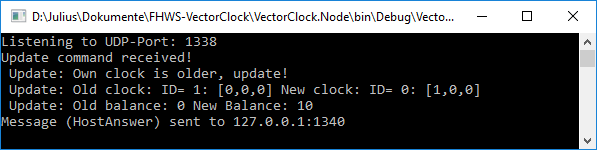
\includegraphics[width=10cm]{nodeWindow.png}
	\caption[Node Window]{Abbildung des Nodefensters. Zwischen den Nodes findet die eigentlichen Kommunikation statt.}
\label{figure:nodeWindow}
\end{figure}
\FloatBarrier

Die Kommunikation zwischen dem Commander und den Nodes wurde mittels UDP realisiert. Die Entscheidung viel auf UDP, da sich dadurch unnötiger Overhead und Programmieraufwand vermeiden lässt, welcher beispielsweise bei TCP angefallen wäre. Der Aufbau einer Nachricht ist in Abbildung \ref{Nachricht} dargestellt. Beim Absenden der Nachricht, egal ob im Commander oder in den Nodes, wird diese serialisiert und per UPD versendet. Im Empfangsfall muss der empfangene Datenstrom wieder deserialisiert und in eine Nachricht umgewandelt werden. 
